% =====================================================================
%  TÓM TẮT ĐỀ TÀI — theo "Hướng dẫn định dạng tóm tắt đề tài" và "Mẫu tóm tắt đề tài"
%   A4; Times New Roman 13pt; dãn dòng single; dãn đoạn trên/dưới 3pt;
%   tên đề tài 16pt, canh giữa, dãn đoạn trên/dưới 12pt;
%   lề trên 3cm, dưới 1,5cm, trái 2,5cm, phải 1,5cm;
%   nội dung 2 cột, khoảng cách 0,7cm; tên hình dưới hình, tên bảng trên bảng;
%   không quá 2 trang.
%  Biên dịch: pdflatex tomtat
% =====================================================================
\documentclass[a4paper,12pt]{article}
\usepackage[fontsize=13pt]{scrextend}
\usepackage[T5]{fontenc}
\usepackage[utf8]{inputenc}
\usepackage[vietnamese]{babel}
\usepackage{mathptmx}
\usepackage[a4paper,top=3cm,bottom=1.5cm,left=2.5cm,right=1.5cm]{geometry}
\usepackage{multicol}
\usepackage{graphicx,booktabs,array,xcolor}
\usepackage[font=small,labelfont=bf,labelsep=period,justification=centering,skip=3pt]{caption}
\usepackage{enumitem}
\usepackage[hidelinks]{hyperref}
% =====================================================================
%  THÔNG TIN CHUNG — dùng chung cho báo cáo, tóm tắt, poster, slide.
%  Sửa ở ĐÂY một lần, mọi tài liệu tự cập nhật khi biên dịch lại.
%  Nguồn: Thuyết minh BM02 (mã số SV2026-474).
% =====================================================================
\newcommand{\tendetai}{Máy bay không người lái tự động theo dõi con người bằng trí tuệ nhân tạo}
\newcommand{\TENDETAI}{MÁY BAY KHÔNG NGƯỜI LÁI TỰ ĐỘNG THEO DÕI CON NGƯỜI BẰNG TRÍ TUỆ NHÂN TẠO}
\newcommand{\madetai}{SV2026-474}
\newcommand{\truong}{Trường Đại học Công nghệ Kỹ thuật Thành phố Hồ Chí Minh}
\newcommand{\TRUONG}{TRƯỜNG ĐH CÔNG NGHỆ KỸ THUẬT TP.HCM}
\newcommand{\khoa}{Đào tạo tiên tiến}
\newcommand{\bomon}{Công nghệ kỹ thuật máy tính}
\newcommand{\nganhhoc}{Công nghệ kỹ thuật máy tính}
\newcommand{\nhomnganh}{Kỹ thuật và Công nghệ}
\newcommand{\loaihinh}{Ứng dụng}

\newcommand{\chunhiem}{Huỳnh Lê Thành Nhân}
\newcommand{\mssvchunhiem}{24119068}
\newcommand{\emailchunhiem}{24119068@student.hcmute.edu.vn}
\newcommand{\dienthoai}{0937395656}

\newcommand{\thanhvien}{Trịnh Trần Quốc Bảo}
\newcommand{\mssvthanhvien}{24119016}
\newcommand{\emailthanhvien}{24119016@student.hcmute.edu.vn}
\newcommand{\dienthoaithanhvien}{0962924006}

\newcommand{\gvhd}{PGS.TS. Lê Mỹ Hà}
\newcommand{\emailgvhd}{halm@hcmute.edu.vn}

% Thông tin cá nhân (chủ nhiệm đề tài cung cấp 16/09/2026).
\newcommand{\gioitinh}{Nam}
\newcommand{\dantoc}{Kinh}
\newcommand{\ngaysinh}{14/08/2006}
\newcommand{\lopchunhiem}{24119FIE4}
\newcommand{\lopthanhvien}{24119FIE4}
\newcommand{\namthu}{3}
\newcommand{\sonamdaotao}{4}

\newcommand{\thangnam}{09/2026}



\usepackage{fancyhdr}
\geometry{headheight=1.5cm,headsep=0.5cm}
\fancypagestyle{hoinghi}{\fancyhf{}\renewcommand{\headrulewidth}{0pt}%
  \fancyhead[L]{\includegraphics[height=1.0cm]{logo_hcmute.png}}%
  \fancyhead[R]{\parbox[b]{9.5cm}{\centering\color[HTML]{C00000}\bfseries HỘI NGHỊ NGHIÊN CỨU KHOA HỌC\\SINH VIÊN NĂM 2026}}}
\setlength{\columnsep}{0.7cm}
\setlength{\parindent}{0.6cm}
\setlength{\parskip}{6pt plus 1pt}   % 3pt trên + 3pt dưới
\linespread{1.0}
\pagestyle{hoinghi}
\setlist{itemsep=0pt,topsep=2pt,parsep=0pt,leftmargin=1.1em}
\captionsetup[table]{position=top}
\captionsetup[figure]{position=bottom}
\addto\captionsvietnamese{\renewcommand{\figurename}{Hình}\renewcommand{\tablename}{Bảng}}
\newcommand{\muc}[1]{\par\vspace{2pt}\noindent\textbf{#1}\par}
\graphicspath{{../hinh/}}

\begin{document}
\begin{center}
\vspace*{-6pt}
{\fontsize{16}{19}\selectfont\bfseries \TENDETAI\par}
\vspace{12pt}
\end{center}

\noindent
\begin{minipage}[c]{3.1cm}\centering
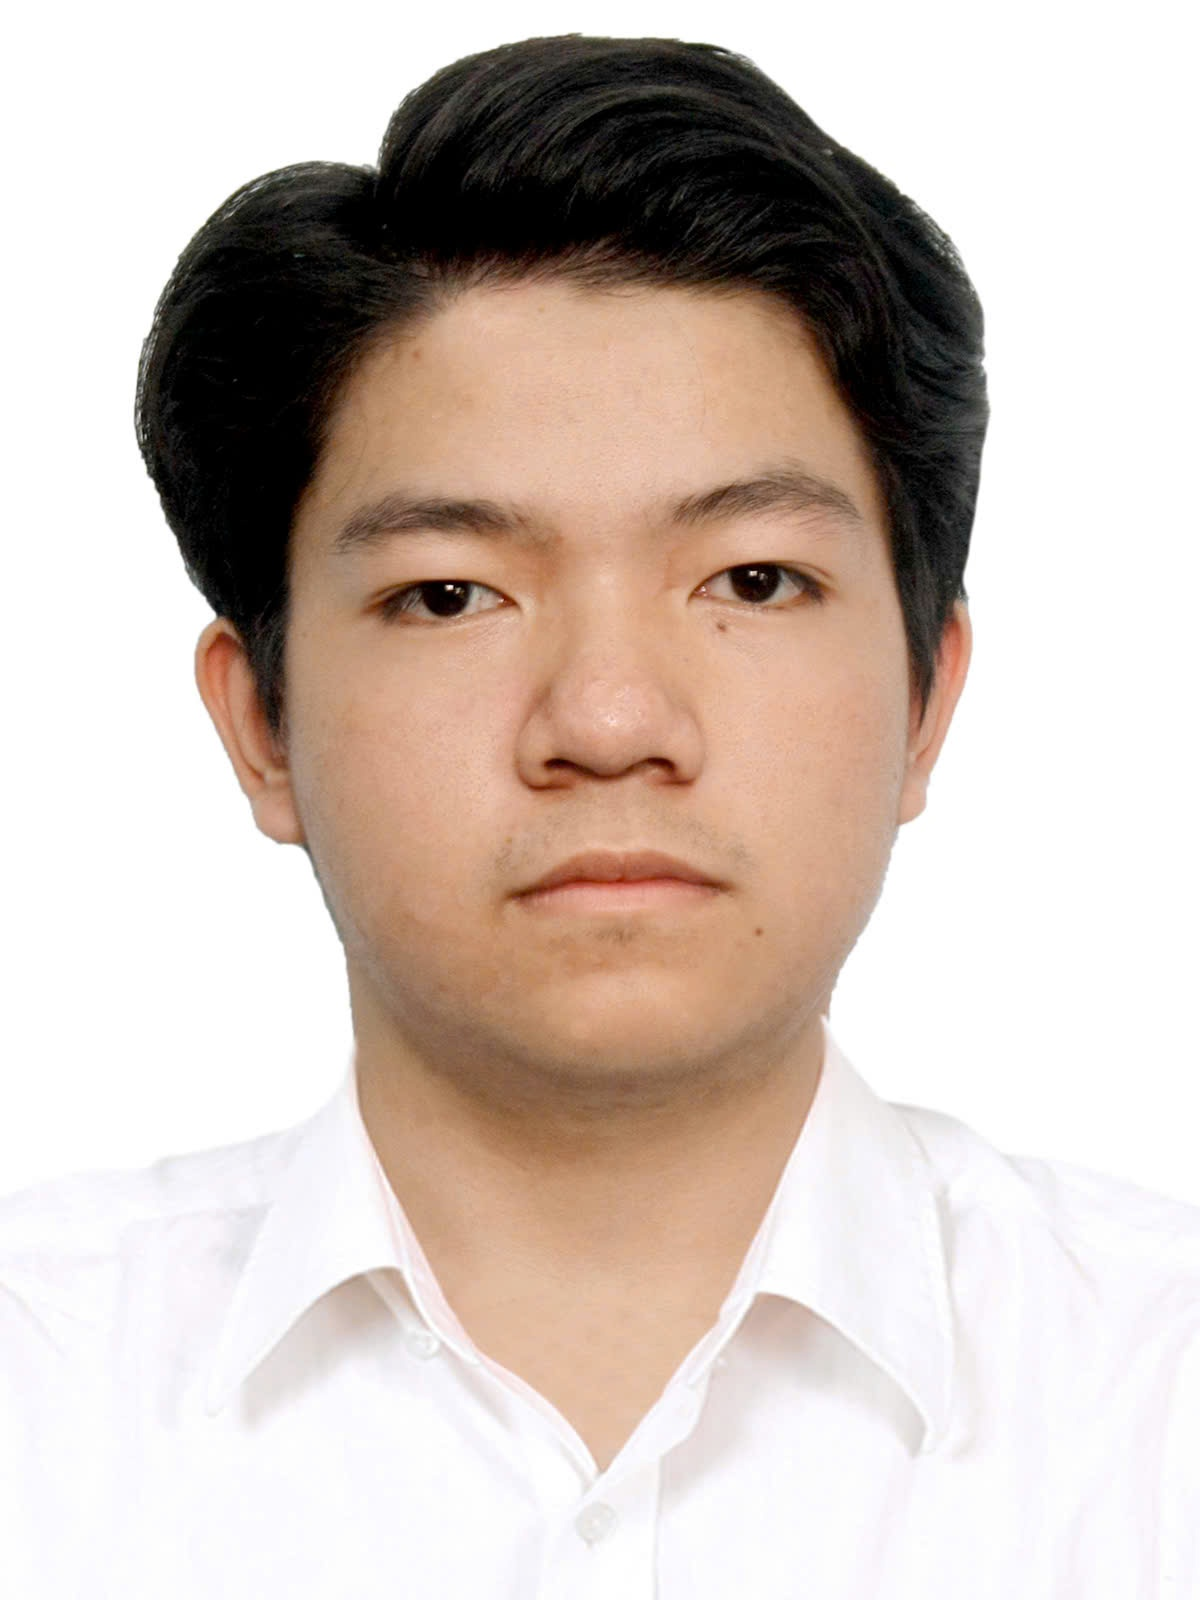
\includegraphics[width=3cm]{anh_3x4.jpg}
\end{minipage}\hspace{0.3cm}%
\begin{minipage}[c]{13.3cm}
\setlength{\tabcolsep}{3pt}
\begin{tabular}{@{}p{5.2cm}p{8.1cm}@{}}
\textbf{\textit{Sinh viên thực hiện chính:}} & \chunhiem\\
\textbf{\textit{Ngày, tháng, năm sinh:}} & \ngaysinh\\
\textbf{\textit{Thành viên đề tài:}} & \thanhvien\\
\textbf{\textit{Giảng viên hướng dẫn:}} & \gvhd\\
\textbf{\textit{Số điện thoại liên lạc:}} & \dienthoai\\
\textbf{\textit{Địa chỉ email:}} & \emailchunhiem\\
\end{tabular}
\end{minipage}

\vspace{4pt}
\noindent\textbf{Tóm tắt nội dung đề tài:}
\vspace{-6pt}

\begin{multicols}{2}

\muc{1. Mục tiêu đề tài}
Máy bay không người lái (UAV) được dùng ngày càng nhiều trong giám sát, cứu hộ và quay phim, nhưng người vận hành vừa phải lái vừa phải giữ đối tượng trong khung hình. Đề tài xây dựng một UAV tự phát hiện và bám theo người, với ba mục tiêu: (i) mô hình trí tuệ nhân tạo nhận dạng người thời gian thực, độ chính xác từ 70\% trở lên; (ii) thuật toán theo dõi giúp máy bay giữ khoảng cách và hướng bay phù hợp; (iii) tích hợp camera -- xử lý ảnh -- điều khiển bay thành hệ thống hoạt động ổn định ngoài thực tế. Toàn bộ xử lý chạy ngay trên máy bay, không cần kết nối Internet.

\muc{2. Tính mới và tính sáng tạo}
Khung máy bay nhiều cánh quạt luôn rung khi bay, làm ảnh bị nhoè, nhiễu và dao động sáng. Bằng một giao thức đo thống nhất, cố định seed ngẫu nhiên và lặp ba lần, nhóm chỉ ra rằng mọi bộ phát hiện nhỏ gọn được thử (YOLOv8/v10/11/26 bản nano, RT-DETR-l) mất 74--83\% độ chính xác khi rung, điều mà các benchmark thông thường không đo. Đề tài đề xuất:
\begin{itemize}
\item \textbf{Mô hình SteadyDet-N} chỉ 1,17 triệu tham số, 4,6 GFLOPs, giữ nhánh độ phân giải cao cho người nhỏ nhưng làm mỏng để chạy trên thiết bị biên.
\item \textbf{Huấn luyện nhận biết rung}: đưa mô hình vật lý của rung vào dữ liệu huấn luyện, không đổi nhãn, \textbf{không tốn chi phí khi suy luận}. Tỷ lệ giữ độ chính xác khi rung tăng từ \textbf{16,8\% lên 36,2\%}.
\item Chứng minh trên phần cứng thật rằng tốc độ trên NPU Hailo-8L phụ thuộc số context: SteadyDet-N nhanh hơn YOLO26-n \textbf{1,70 lần}.
\item Lớp an toàn theo nguyên tắc người lái luôn giữ quyền chế độ bay, được khoá bằng kiểm thử tự động.
\end{itemize}

\muc{3. Kết quả nghiên cứu}
Hệ thống gồm Raspberry Pi~5 gắn NPU Hailo-8L, camera USB và bộ điều khiển bay Pixhawk~6C chạy ArduPilot. Chuỗi xử lý: phát hiện người (SteadyDet-N INT8) $\rightarrow$ theo vết OC-SORT $\rightarrow$ khoá mục tiêu $\rightarrow$ ước lượng khoảng cách theo mô hình camera lỗ kim và bộ lọc Kalman $\rightarrow$ ba bộ PID $\rightarrow$ lớp an toàn $\rightarrow$ lệnh vận tốc MAVLink 30\,Hz ở chế độ GUIDED.

\noindent\begin{minipage}{\linewidth}
\centering
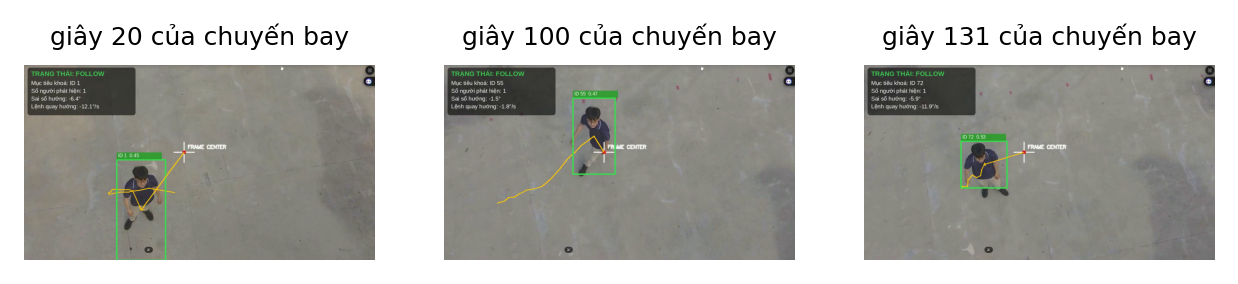
\includegraphics[width=\linewidth]{vongbam_khung.png}
\captionof{figure}{Vòng bám người trên video bay thử ở độ cao khoảng 6\,m}
\end{minipage}
\vspace{4pt}

\noindent\begin{minipage}{\linewidth}
\centering
\captionof{table}{Kết quả chính đo trên phần cứng thật}
\footnotesize
\renewcommand{\arraystretch}{1.1}
\setlength{\tabcolsep}{3pt}
\begin{tabular}{@{}>{\raggedright\arraybackslash}p{4.75cm}r@{}}
\toprule
\textbf{Chỉ số} & \textbf{Kết quả}\\
\midrule
AP@0,5 trên dữ liệu bay thật (INT8) & \textbf{0,917}\\
F1 / recall / precision & 0,880 / 0,837 / 0,928\\
Tốc độ đầu-cuối trên máy bay & \textbf{30,0 FPS}\\
Độ trễ trung vị / p99 & 32,04 / 36,15\,ms\\
Suy luận NPU @320 / @640 & 112,55 / 63,66 FPS\\
retain khi rung (gốc $\rightarrow$ đề xuất) & 16,8 $\rightarrow$ \textbf{36,2\%}\\
AP ở mức rung bay tiến & tăng \textbf{4,2 lần}\\
Khứ hồi lệnh MAVLink p50 / p99 & 4,75 / 7,73\,ms\\
Vòng bám trên video bay thử: giữ mục tiêu & 83,5\% thời gian\\
Sai số hướng khi bám (trung vị) & 5,5$^\circ$\\
\bottomrule
\end{tabular}
\end{minipage}
\vspace{4pt}

Mô hình trên máy bay đạt \textbf{AP@0,5 = 91,7\%}, vượt chỉ tiêu 70\% của thuyết minh. Khi rung, SteadyDet-N là mô hình nhỏ và rẻ nhất nhưng vượt cả bốn mô hình YOLO bản nano, và vượt RT-DETR-l (lớn gấp 28 lần) ở mức rung của bay tiến thông thường. Trên dữ liệu bay thật, xử lý rung làm độ khít hộp AP@0,75 tăng khoảng 80\%. Chương trình điều khiển có theo vết, khoá và tìm lại mục tiêu, thang an toàn khi mất mục tiêu và bảng giám sát web; hệ thống được kiểm thử qua bảy tầng từ kiểm thử tự động tới bay thử ngoài bãi. Chạy trên video bay thử, vòng bám khoá và giữ được người đi bộ trong 83,5\% thời gian.

\noindent\begin{minipage}{\linewidth}
\centering
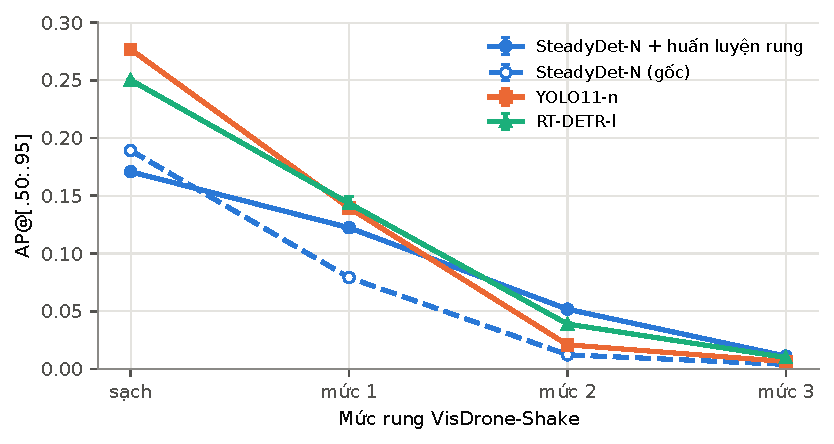
\includegraphics[width=\linewidth]{duong_cong_rung.pdf}
\captionof{figure}{AP theo mức rung: sau huấn luyện nhận biết rung, SteadyDet-N vượt YOLO11-n và RT-DETR-l từ mức 2}
\end{minipage}
\vspace{4pt}

\muc{4. Đóng góp về mặt kinh tế -- xã hội, giáo dục và đào tạo, an ninh quốc phòng và khả năng áp dụng thực tế}
Hệ thống dùng linh kiện phổ thông, xử lý hoàn toàn trên máy bay nên hoạt động được ở vùng không có sóng di động, phù hợp tìm kiếm cứu nạn sau thiên tai, giám sát an ninh, tuần tra khu vực và quay phim tự động. Phương pháp huấn luyện nhận biết rung chỉ thay đổi dữ liệu huấn luyện, áp dụng được cho camera trên robot, xe tự hành mà không cần gimbal chống rung đắt tiền. Về đào tạo, đề tài cung cấp quy trình trọn vẹn, tái lập được từ dữ liệu, huấn luyện, lượng tử hoá, triển khai trên NPU tới điều khiển bay, dùng làm học liệu cho các học phần thị giác máy tính, hệ thống nhúng và điều khiển tự động.

\muc{5. Công bố khoa học của SV từ kết quả nghiên cứu của đề tài}
Chưa có.
\end{multicols}
\end{document}
